\documentclass[twocolumn, amsmath, amsfonts, amssymb]{aastex62}
\usepackage{mathtools}
\usepackage{bm}
\newcommand{\vdag}{(v)^\dagger}
\newcommand\aastex{AAS\TeX}
\newcommand\latex{La\TeX}

\newcommand{\Div}[1]{\ensuremath{\nabla\cdot\left( #1\right)}}
\newcommand{\DivU}{\ensuremath{\nabla\cdot\bm{u}}}
\newcommand{\angles}[1]{\ensuremath{\left\langle #1 \right\rangle}}
\newcommand{\KS}[1]{\ensuremath{\text{KS}(#1)}}
\newcommand{\KSstat}[1]{\ensuremath{\overline{\text{KS}(#1)}}}
\newcommand{\grad}{\ensuremath{\nabla}}
\newcommand{\RB}{Rayleigh-B\'{e}nard }
\newcommand{\stressT}{\ensuremath{\bm{\bar{\bar{\Pi}}}}}
\newcommand{\lilstressT}{\ensuremath{\bm{\bar{\bar{\sigma}}}}}
\newcommand{\nrho}{\ensuremath{n_{\rho}}}
\newcommand{\approptoinn}[2]{\mathrel{\vcenter{
	\offinterlineskip\halign{\hfil$##$\cr
	#1\propto\cr\noalign{\kern2pt}#1\sim\cr\noalign{\kern-2pt}}}}}

\newcommand{\appropto}{\mathpalette\approptoinn\relax}



%% Tells LaTeX to search for image files in the 
%% current directory as well as in the figures/ folder.
\graphicspath{{./}{figs/}}


\received{\today}
\revised{\today}
\accepted{\today}
\submitjournal{ApJ}

\shorttitle{Small name}
\shortauthors{Anders, Manduca, and Brown}

\begin{document}

\title{Controlling the rotational constraint in stratified, compressible convection}

\correspondingauthor{Evan H. Anders}
\email{evan.anders@colorado.edu}

\author{Evan H. Anders}
\affil{University of Colorado -- Boulder}
\author{Katie Manduca}
\affil{University of Colorado -- Boulder}
\author{Benjamin P. Brown}
\affil{University of Colorado -- Boulder}


\begin{abstract}
\end{abstract}

\keywords{convection --- happy caterpillars}

%%%%% Body of the paper
\section{Introduction}
\label{sec:intro}
Recent work by \cite{featherstone&hindman2016} needs to be talked about.
Rotating dynamo stuff \cite{busse2002, brown&all2008, brown&all2010, brown&all2011} 
Papers on rotating RB convection that might matter:
\cite{hathaway&somerville1983, julien&all1996, zhong&all2009, julien&all2012, stellmach&all2014}.
Papers on rotating stratified f-planes that might matter:
\cite{brummell&all1996, brummell&all1998, calkins&all2015a}.  Honestly, most stratified, rotating sims
seem to avoid simplicities (like the f-plane) as though they were the plague.

\section{Experiment} 
\label{sec:experiment}
We study fully compressible, stratified 
convection as we previously did in \cite{anders&brown2017}, with 
the inclusion of rotation. We study an ideal gas whose
equation of state is $P = R \rho T$ and with an adiabatic
index $\gamma = 5/3$. We nondimensionalize the atmosphere such that
$R = 1$ and $P = \rho = T = 1$ at the top of the domain.
The initial stratification is polytropic, such that
\begin{equation}
\begin{split}
\rho_0(z) &= (1 + L_z - z)^m, \\
T_0(z)    &= (1 + L_z - z),
\label{eqn:polytrope}
\end{split}
\end{equation}
where $m$ is the polytropic index,
$z$ increases upwards in the range $z = [0, L_z]$, and
$L_z \equiv e^{n_\rho/m} - 1$ is the depth of the atmosphere,
where $n_\rho$ specifies the number of density scale heights that the
atmosphere spans. We specify the instability of the atmosphere
through the superadiabatic excess, $\epsilon = m - m_{ad}$, where
$m_{ad} = (\gamma-1)^{-1}$ is the adiabatic polytropic index, and
$\epsilon$ controls the Mach number of the flows \citep{anders&brown2017}.
The domain is a 3D cartesian box whose horizontal extent is in the range
$x, y = [0, AL_z]$, where $A$ is the aspect ratio of the domain.
As has been studied previously by e.g., \cite{julien&all1996, brummell&all1996}, 
we study a domain in which the
gravity and rotational vector are antiparallel, $\bm{g} = -g\hat{z}$,
and $\bm{\Omega} = \Omega \hat{z}$.

We evolve the velocity ($\bm{u}$), temperature, and log density according to the
Fully Compressible Navier-Stokes equations,
\begin{align}
&\begin{aligned}
&\frac{\partial \ln\rho}{\partial t} + \grad\cdot\bm{u} 
    = -\bm{u}\cdot\grad\ln\rho,
	\label{eqn:continuity_eqn}
\end{aligned}\\
&\begin{aligned}
\frac{\partial\bm{u}}{\partial t} + 2\bm{\Omega}&\times\bm{u} + \grad T - 
\nu\grad\cdot\lilstressT - \lilstressT\cdot\grad\nu = \\
&-\bm{u}\cdot\grad\bm{u} - T\grad\ln\rho + \bm{g} + 
\nu\lilstressT\cdot\grad\ln\rho,
\label{eqn:momentum_eqn}
\end{aligned}\\
&\begin{aligned}
\frac{\partial T}{\partial t} -\frac{1}{c_V}\left(\right.\chi&\left.
    \grad^2 T + \grad T\cdot\grad\chi\right) = \\
	&-\bm{u}\cdot\grad T - (\gamma-1)T\grad\cdot{\bm{u}} \\
	&+ \frac{1}{c_V}\left(\chi\grad T \cdot\grad\ln\rho +
	\nu\left[\lilstressT\cdot\nabla\right]\cdot\bm{u}\right), 
	\label{eqn:energy_eqn}
\end{aligned}
\end{align}
with the viscous stress tensor given by
\begin{equation}
\sigma_{ij} \equiv \left(\frac{\partial u_i}{\partial x_j} + 
\frac{\partial u_j}{\partial x_i} - \frac{2}{3}\delta_{ij}\grad\cdot\bm{u}\right).
	\label{eqn:stress_tensor}
\end{equation}

The kinematic viscosity, $\nu$, thermal diffusivity, $\chi$, and strength of
rotation $\Omega$ are set at the top of the domain by the Rayleigh number
(Ra), Prandtl number (Pr), and Taylor number (Ta),
\begin{equation}
\text{Ra} = \frac{g L_z^3 \Delta S / c_P}{\nu \chi}, \,\,\,
\text{Pr} = \frac{\nu}{\chi}, \,\,\,
\text{Ta} = \left(\frac{2 \Omega L_z^2}{\nu}\right)^2,
\end{equation}
where $\Delta S = \epsilon n_\rho / m$ is the specific entropy difference between
$z = 0$ and $z = L_z$, and the specific heat at constant pressure is $c_P$.




We measure the resulting Rossby number, Nusselt number, and Reynolds number of all flows in order to
understand the various regimes of convection which are open to us.

\begin{figure}[h]
%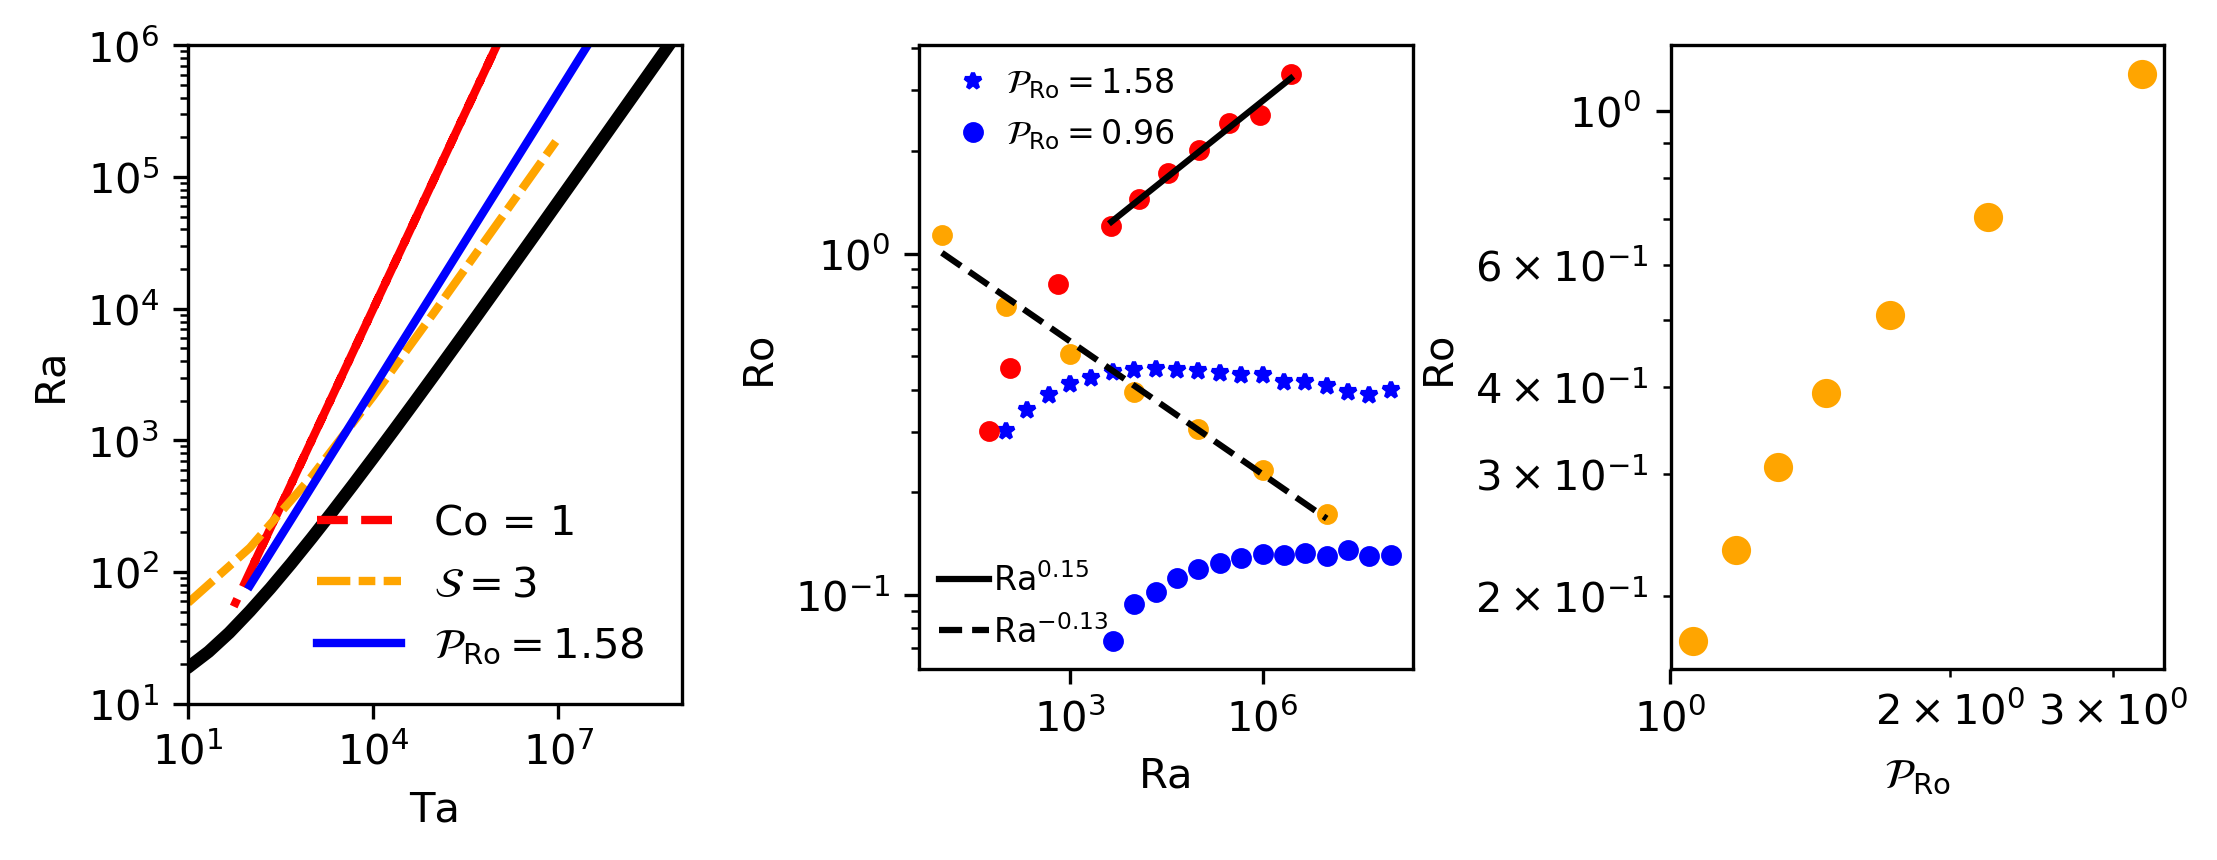
\includegraphics[width=\textwidth]{./figs/parameter_space.png}
\caption{(a) The critical Rayleigh number, as a function of the Taylor number, 
is plotted as a solid black line. Paths of constant Convective Rossby Number
(red dashed line), constant supercriticality (orange dashed line), and 
COPRIME (blue solid line) are shown through parameter space. (b) Evolved
Rossby number is plotted vs. Taylor number along multiple constant COPRIME
paths, such as the solid blue line in (a). 
After a sharp increase at low Ta, the evolved Rossby number flattens
out and stays nearly constant across orders of magnitude of Ta.
\label{fig:parameter_space} }
\end{figure}



\section{Results \& Discussion}
\label{sec:results}
This is where figures go and other important things that we like to talk about.


\begin{figure}[h]
%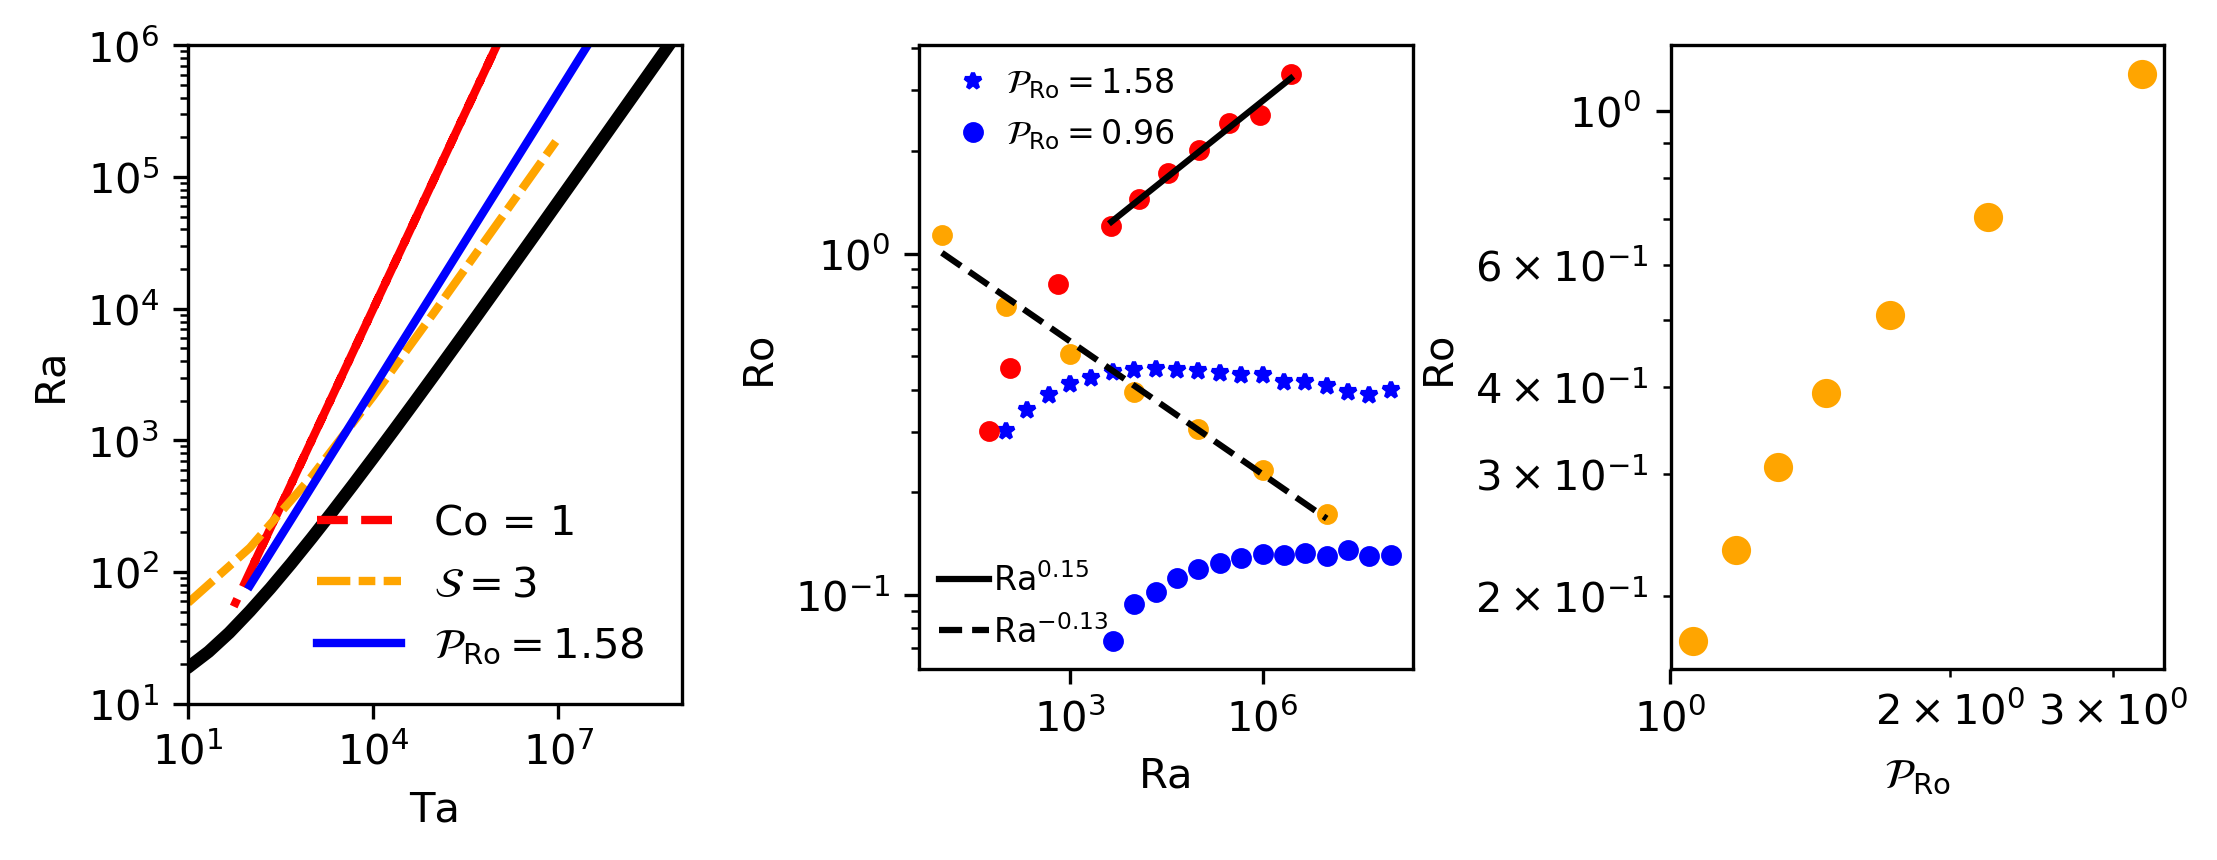
\includegraphics[width=\textwidth]{./figs/parameter_space.png}
\caption{(a) Evolved Nusselt number vs. Rayleigh number / Ra\_crit along constant
COPRIME paths. A classic scaling law of $Nu \propto Ra^{2/7}$ is observed.
(b) Evolved Reynolds number vs. Rayleigh number / Ra\_crit along constant COPRIME paths.
A classic scaling law of $Re \propto Ra^{1/2}$ is observed. These laws are
reminiscent of standard scaling laws of Re and Nu in non-rotational convection
(SOURCES SOURCES SOURCES). This suggests that at fixed Rossby number on
a constant COPRIME path (Fig. \ref{fig:parameter_space}), varying the Rayleigh
number affects the evolved dynamics in a manner similar to a nonrotating fluid.
\label{fig:nu_and_re} }
\end{figure}

\begin{figure}[h]
%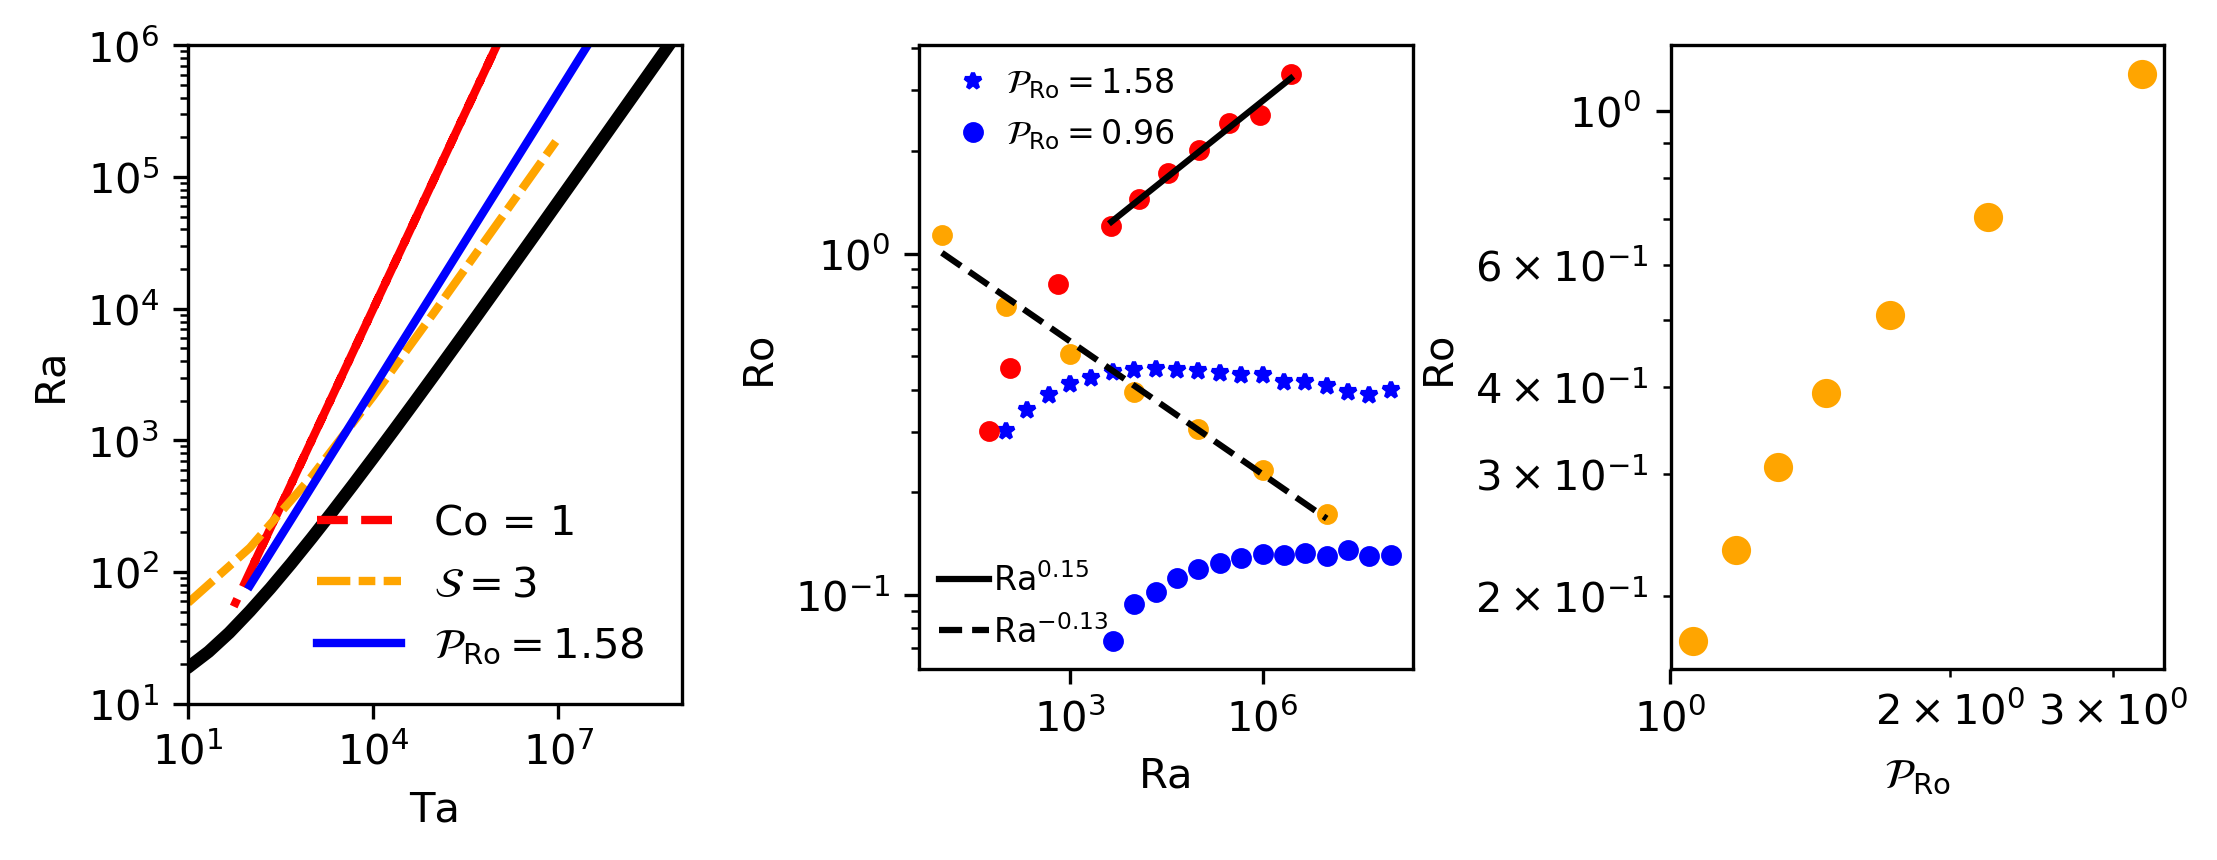
\includegraphics[width=\textwidth]{./figs/parameter_space.png}
\caption{ Here's some pretty plots, we'll figure out what we plot later.
\label{fig:pretty_convection} }
\end{figure}

\begin{figure}[h]
%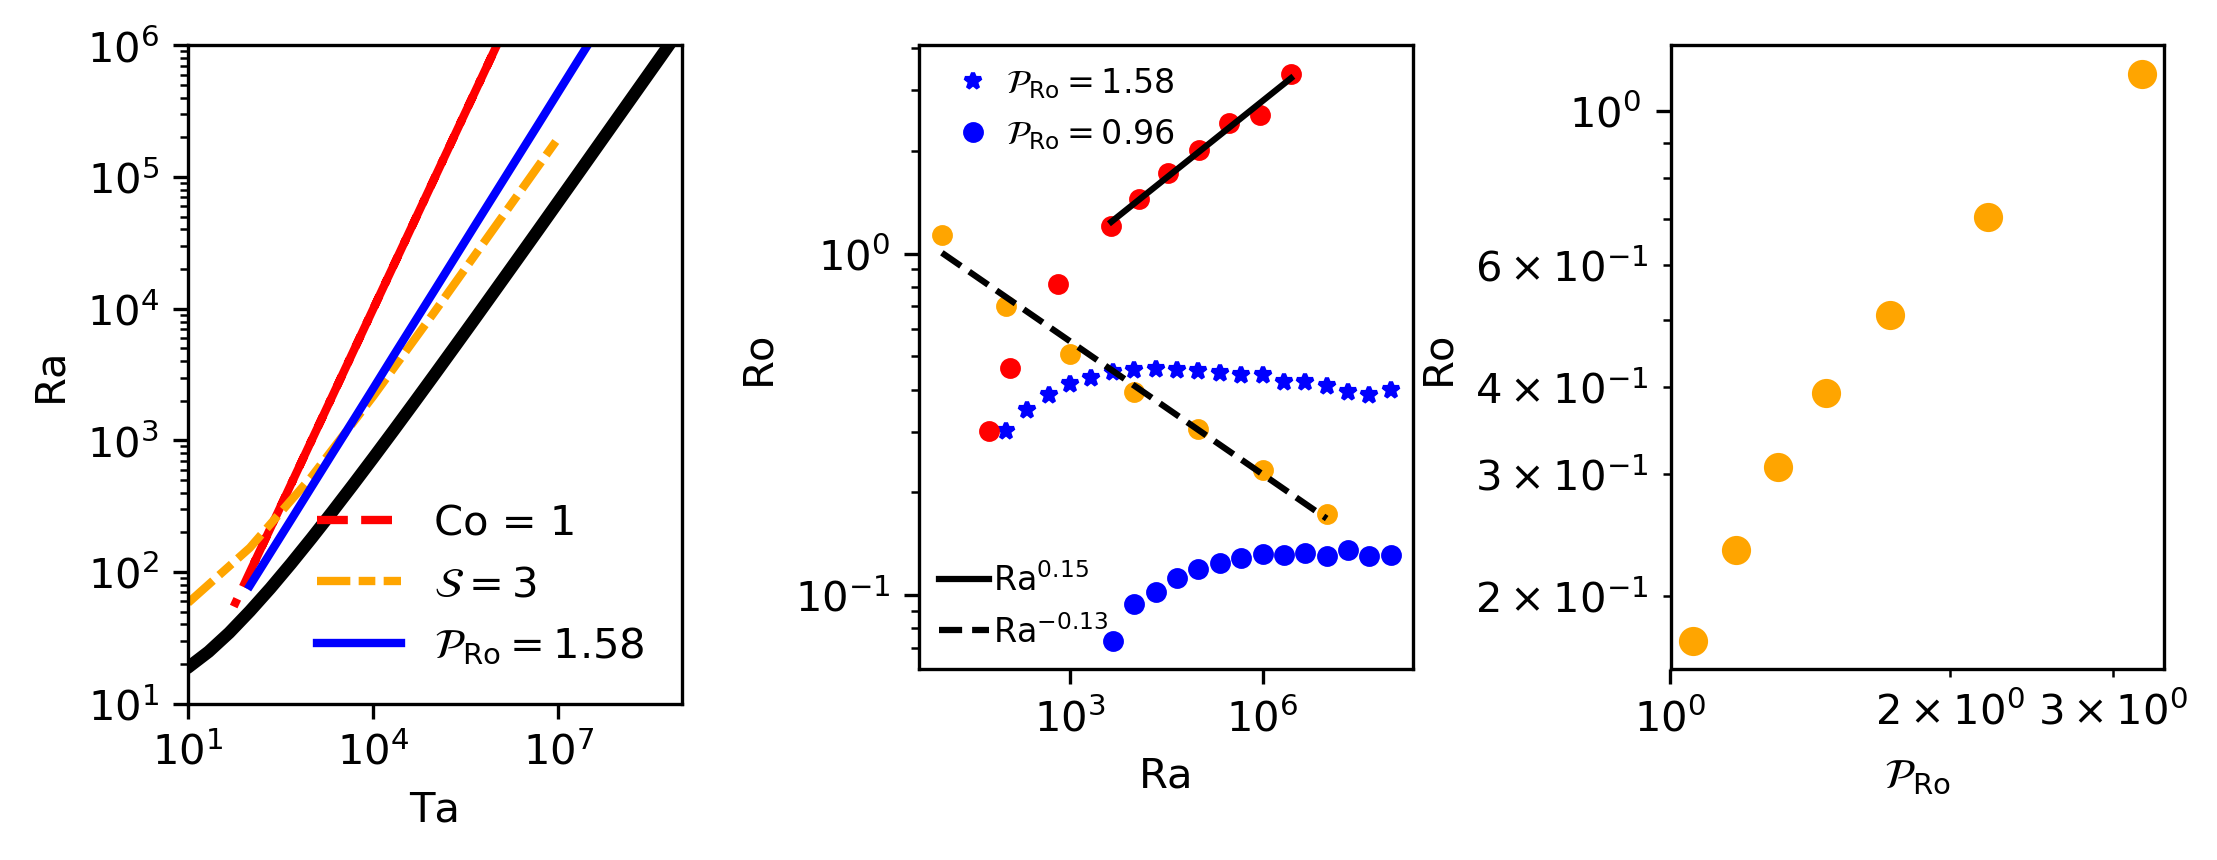
\includegraphics[width=\textwidth]{./figs/parameter_space.png}
\caption{(a) Horizontally-averaged profiles of the Rossby number are shown
vs. z for a constant COPRIME = X. (b) Horizontally-averaged profiles of 
the entropy gradient are shown vs. z for a constant COPRIME = X.
(c) Vorticity boundary layer thickness normalized by entropy boundary layer
thickness as a function of Ta/Ta\_crit for multiple COPRIME paths.
When this measure is $\gg 1$, we expect the flows to be buoyancy dominated,
when it is $\ll 1$, we expect the flows to be rotationally dominated,
and when it is $\sim 1$, we anticipate that both effects are very important.
\label{fig:profiles_and_bls} }
\end{figure}







\subsection{acknowledgements}
EHA acknowledges the support of the University of Colorado's George 
Ellery Hale Graduate Student Fellowship.
This work was additionally supported by  NASA LWS grant number NNX16AC92G.  
Computations were conducted 
with support by the NASA High End Computing (HEC) Program through the NASA 
Advanced Supercomputing (NAS) Division at Ames Research Center on Pleiades
with allocations GID s1647.
We thank  Jeff Oishi for many useful discussions. 

\bibliography{biblio.bib}
\end{document}
